\section{Transformer}
\label{sec:transformer}
\begin{frame}
\frametitle{Transformer}
\begin{figure}
    % \begin{minipage}[t]{0.5\textwidth}
    %   \centering
    %   %Scaled Dot-Product Attention \\
    %   Transformer model architecture \\
    %   \vspace{0.1cm}
    %   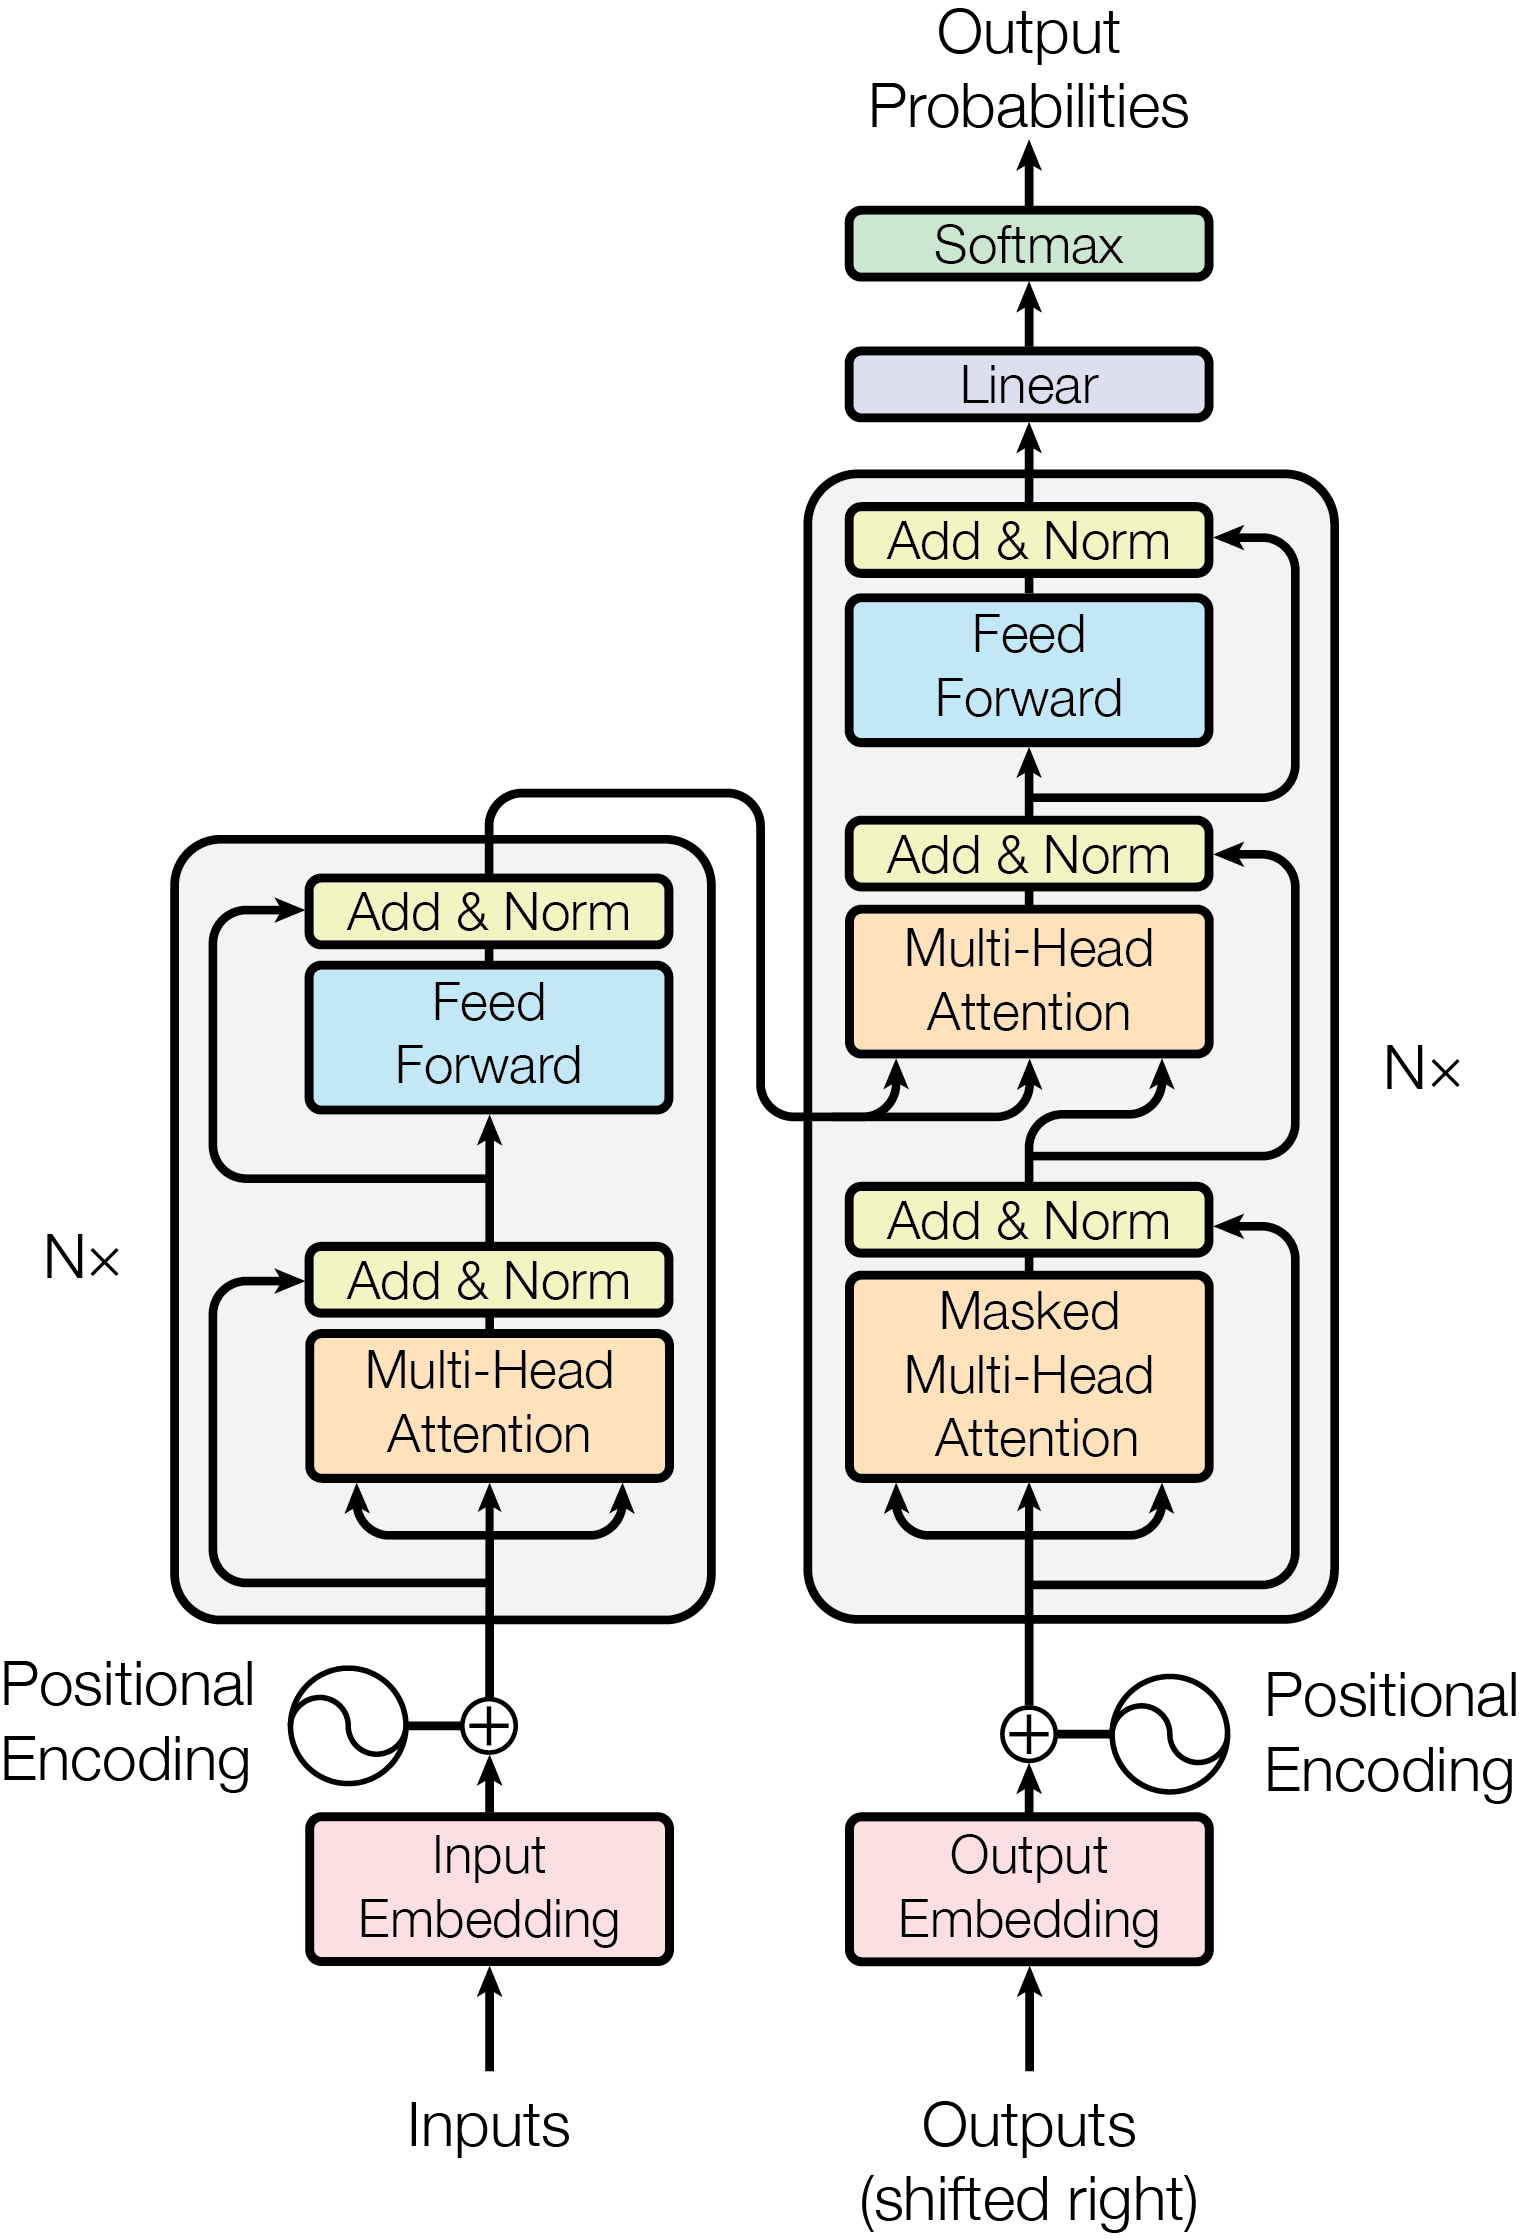
\includegraphics[scale=0.35]{./tokenformer-paper/Figures/ModalNet-21}
    % \end{minipage}\hfill
    \begin{minipage}[t]{0.5\textwidth}
      \centering 
      Multi-Head Attention \\
      \vspace{0.1cm}
      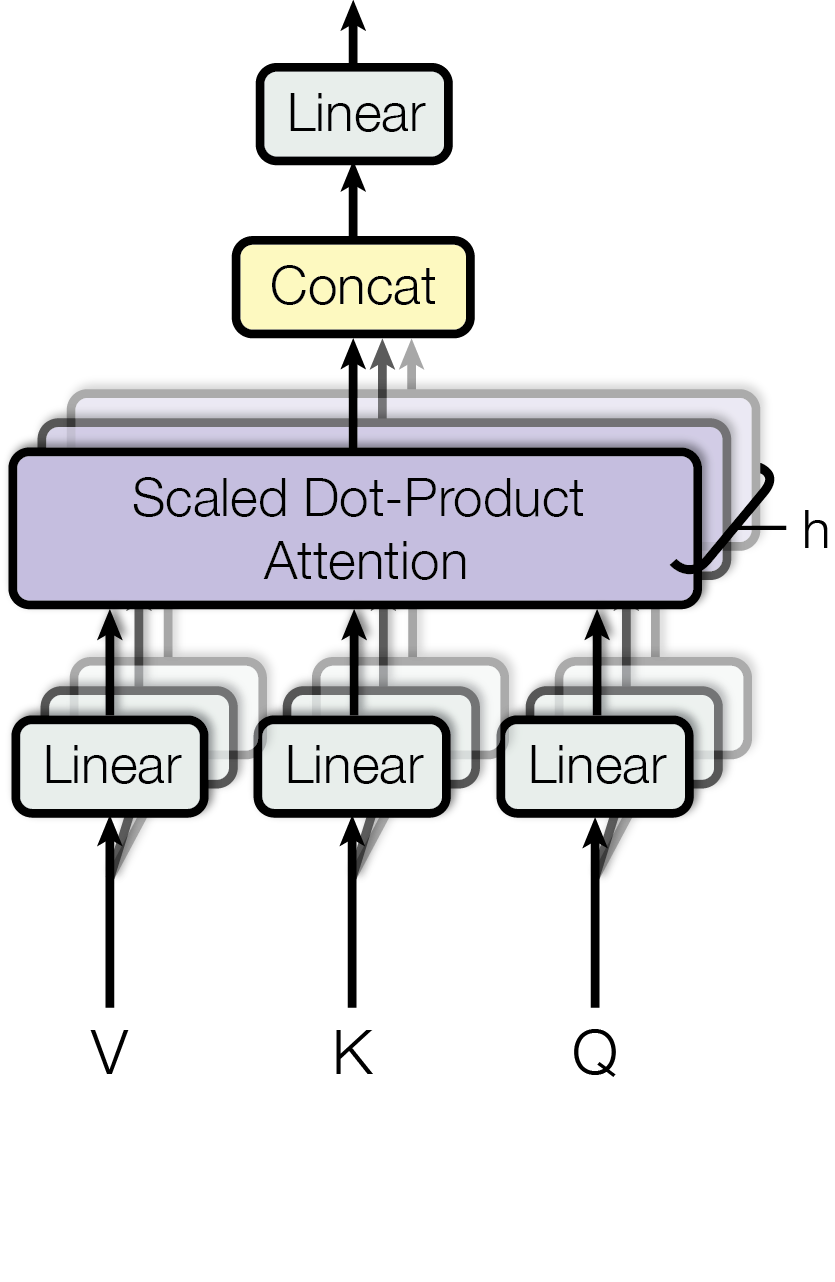
\includegraphics[scale=0.6]{./tokenformer-paper/Figures/ModalNet-20}  
    \end{minipage}\hfill
    \begin{minipage}[t]{0.5\textwidth}
      %\centering 
       Input tokens: $X\in\mathbb{R}^{T\times d}$ \\
       \begin{equation}
        Q = X\cdot W^Q, \quad K = X\cdot W^K, \quad V = X\cdot W^V;
       \end{equation}
       $W^Q, W^K \in\mathbb{R}^{d\times d_k}, W^V \in\mathbb{R}^{d\times d_v}$. \\
       \begin{equation}
        \text{Attention}(Q,K,V)=\text{softmax}(\frac{QK^T}{\sqrt{d_k}})V.
       \end{equation}
       Output: $$O=X_{\text{att}}\cdot W^O, \quad W^O \in\mathbb{R}^{d_v\times d}.$$
       FFN: $$X_{\text{ffn}} = \text{Activation}(O\cdot W_1 + b_1)W_2 + b_2.$$
       $W_1 \in \mathbb{R}^{d\times d_{\text{ffn}}},
       W_2 \in \mathbb{R}^{d_{\text{ffn}}\times d}.$
    \end{minipage}
    
    
      % \centering
    
      %\caption{(left) Scaled Dot-Product Attention. (right) Multi-Head Attention consists of several attention layers running in parallel.}
      \label{fig:multi-head-att}
    \end{figure}
    
\end{frame}
